\documentclass{article}
\usepackage[left=2cm, right=2cm]{geometry}
\usepackage{amsmath}
\usepackage{amssymb}
\usepackage{fancyvrb}
\usepackage{xcolor}

\usepackage{graphicx}
\usepackage{enumitem}
\usepackage{tikz}
\usepackage{pgfplots}
\usepackage{hyperref}
\setlength\parindent{0pt}
% \hypersetup{
%    colorlinks,
%    citecolor=green,
%    filecolor=black,
%    linkcolor=blue,
%    urlcolor=blue
%}
\begin{document}
\title{\vspace{-2.0cm} LBA}
\author{Jacob Puthipiroj, Uyen Nguyen}
%\date{}
\maketitle

\begin{abstract}
	In this paper, we establish a link between household gun ownership and teen suicide rates. Methodologically we establish this link through a simple linear regression of household gun ownership at the state level of suicides, and then a multiple regression, with the inclusion of suicide attempts as an additional explanatory variable. According to our model,  we predict that each 1\% absolute increase in household gun ownership is associated with a 2.15\% relative increase in youth suicides. Because guns are a much more lethal form of suicide attempt, a policy restricting the overall availability of guns should decrease not the number of suicide attempts, but the number of suicides overall. We therefore immediately urge policymakers to restrict the possession of firearms.
\end{abstract}

\subsection*{Context \& Background}
The United States is the only country in the world with more guns than people. The United States has a unique relationship with guns, starting with the second amendment, the right to bear arms, being written into the Constitution within 20 years of the founding of the country. In modern times, gun laws in the US have come under heated scrutiny, with advocates of gun control often claiming a link between gun ownership and homicide. In this paper, we instead argue for greater gun control by establishing a link between gun ownership and teen (defined as under 18 suicide). \\

We do not attempt to argue that guns cause suicide attempts. We instead argue that \textit{the prevalence of guns makes preexisting suicide attempts more successful}. We explicitly acknowledge that a reduction of guns does not and will not address the root causes that drive teens to contemplate, plan for, and attempt suicide. We predict, however, that a reduction of guns will likely reduce the number of teen funerals in the US. We argue for an immediate treatment of the symptom, rather than the ``root cause" of teen suicide, simply as a matter of urgency and practicality. In our analysis, we compare simple regressions of suicide rates on gun ownership, and multiple regressions of suicide rates on gun ownership and suicide attempts.\footnote{\#causaleffect: we define and explain causality in the context of gun ownership on teen suicide rate, identifying possible mechanisms, justifying our application (here and in the limitations section), and explain why it may not be possible to elicit causal relationships from cross-sectional data}\\

\subsection*{Data}

Data was collected for each of the 50 States of the US on 3 variables: the log number of suicides per 100,000, ln(suicides); the percentage of households with gun ownership, and the percentage of youths who reported having attempted suicide. \footnote{\#data: We explain the data structures of the variables (the suicide rate, household gun ownership, and suicide attempts) involved, explaining the data collection process, and why they are the best data.}
\begin{enumerate}
	\item Data for the first variable was taken from the CDC's Injury Statistics Query and Reporting System. Data comes from death certificates collected as part of the national vital statistics program. Since the CDC does not report suicide rates based on less than 10 deaths which generates stable estimates of suicide rates by aggregating across the 11th studies from 2005 to 2015. For 2 other states, Hawaii and Rhode Island, data was aggregated from 2003 to 2015 instead because of the low numbers of annual suicides. The variables originally had high skew (1.6) and kurtosis (5.4), which was reduced to acceptable levels (skew = 0.5, kurtosis = 3.1) after being logged.
	\item Data for the second variable was taken from the 2004 Behavioral Risk Factor Surveillance System Survey. The BRFSS has not assessed gun ownership at the state level since 2004, and so there are no contemporaneous sources on state-level data. However using only data from 2004 (as a cross-sectional study) in the independent variable has the benefit of ruling out reverse causation, in which gun ownership levels them selves are responding to changes in youth suicide rates as the dependent variable.
	\item Data for the third variable was taken from the youth risk behavior surveillance system (YRBSS), a biennial national school survey administered every two years by the CDC. The relevant question on the survey was, ``have you attempted suicide one or more times during the 12 months before the survey?" We averaged the state-wide numbers across the 5 surveys from 2005-2015. Three states; Minnesota, Oregon and Washington did not participate in the YRBSS, and so are not used in the multiple regression.

\end{enumerate}

\subsection*{Findings}

The variable log suicide and the variable ownership was moderately correlated, with $R^2=0.55$. As a trend, states with high gun ownership's also had had levels of teen suicide rate. In our simple linear regression,  we obtain a coefficient of 0.02134, indicating a roughly $e^{0.02134}-1=2.15 \%$ (relative) increase in teen suicide rates for every 1\% (absolute) increase in household gun ownership percentages. In other studies, which attempt to rigorously separate the magnitude of the effect of guns, such as through linear regression in Knopov et al (2018), important explanatory variables for teen suicide have included psychopathological factors (Cash and Bridge, 2009), race, alcohol and drug use, family make up, and sociodemographic variables, such as poverty, divorce, education, unemployment, and urbanicity (Anestis), and findings were similar, but even higher numbers were obtained. \\

\begin{figure*}[h]
\centering
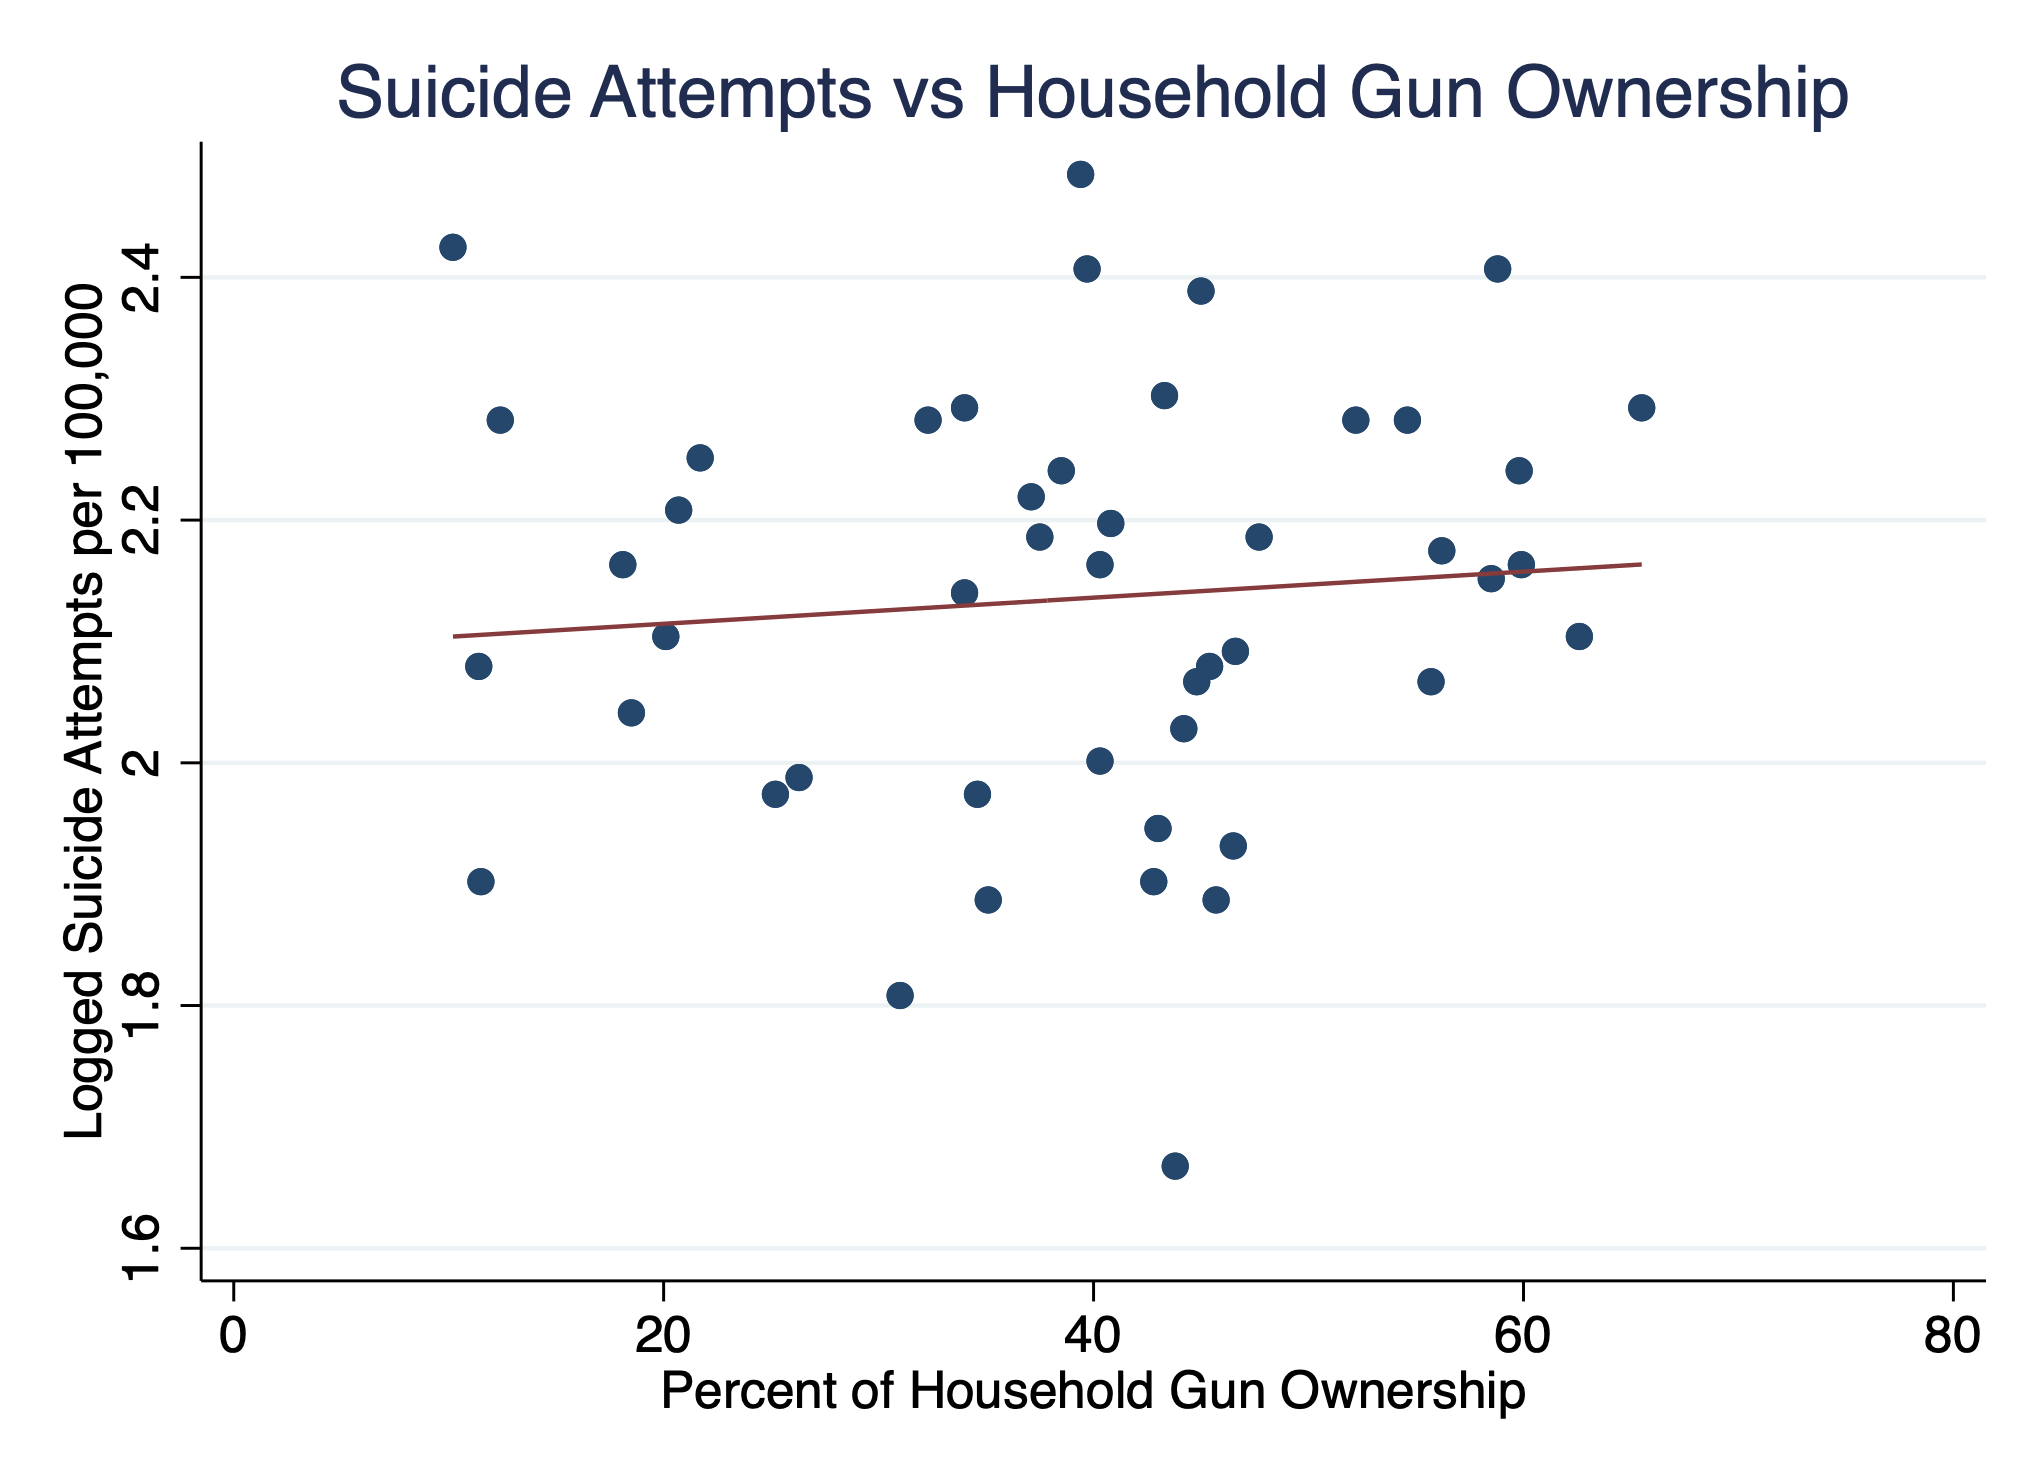
\includegraphics[width=8.5cm]{graph1.png}
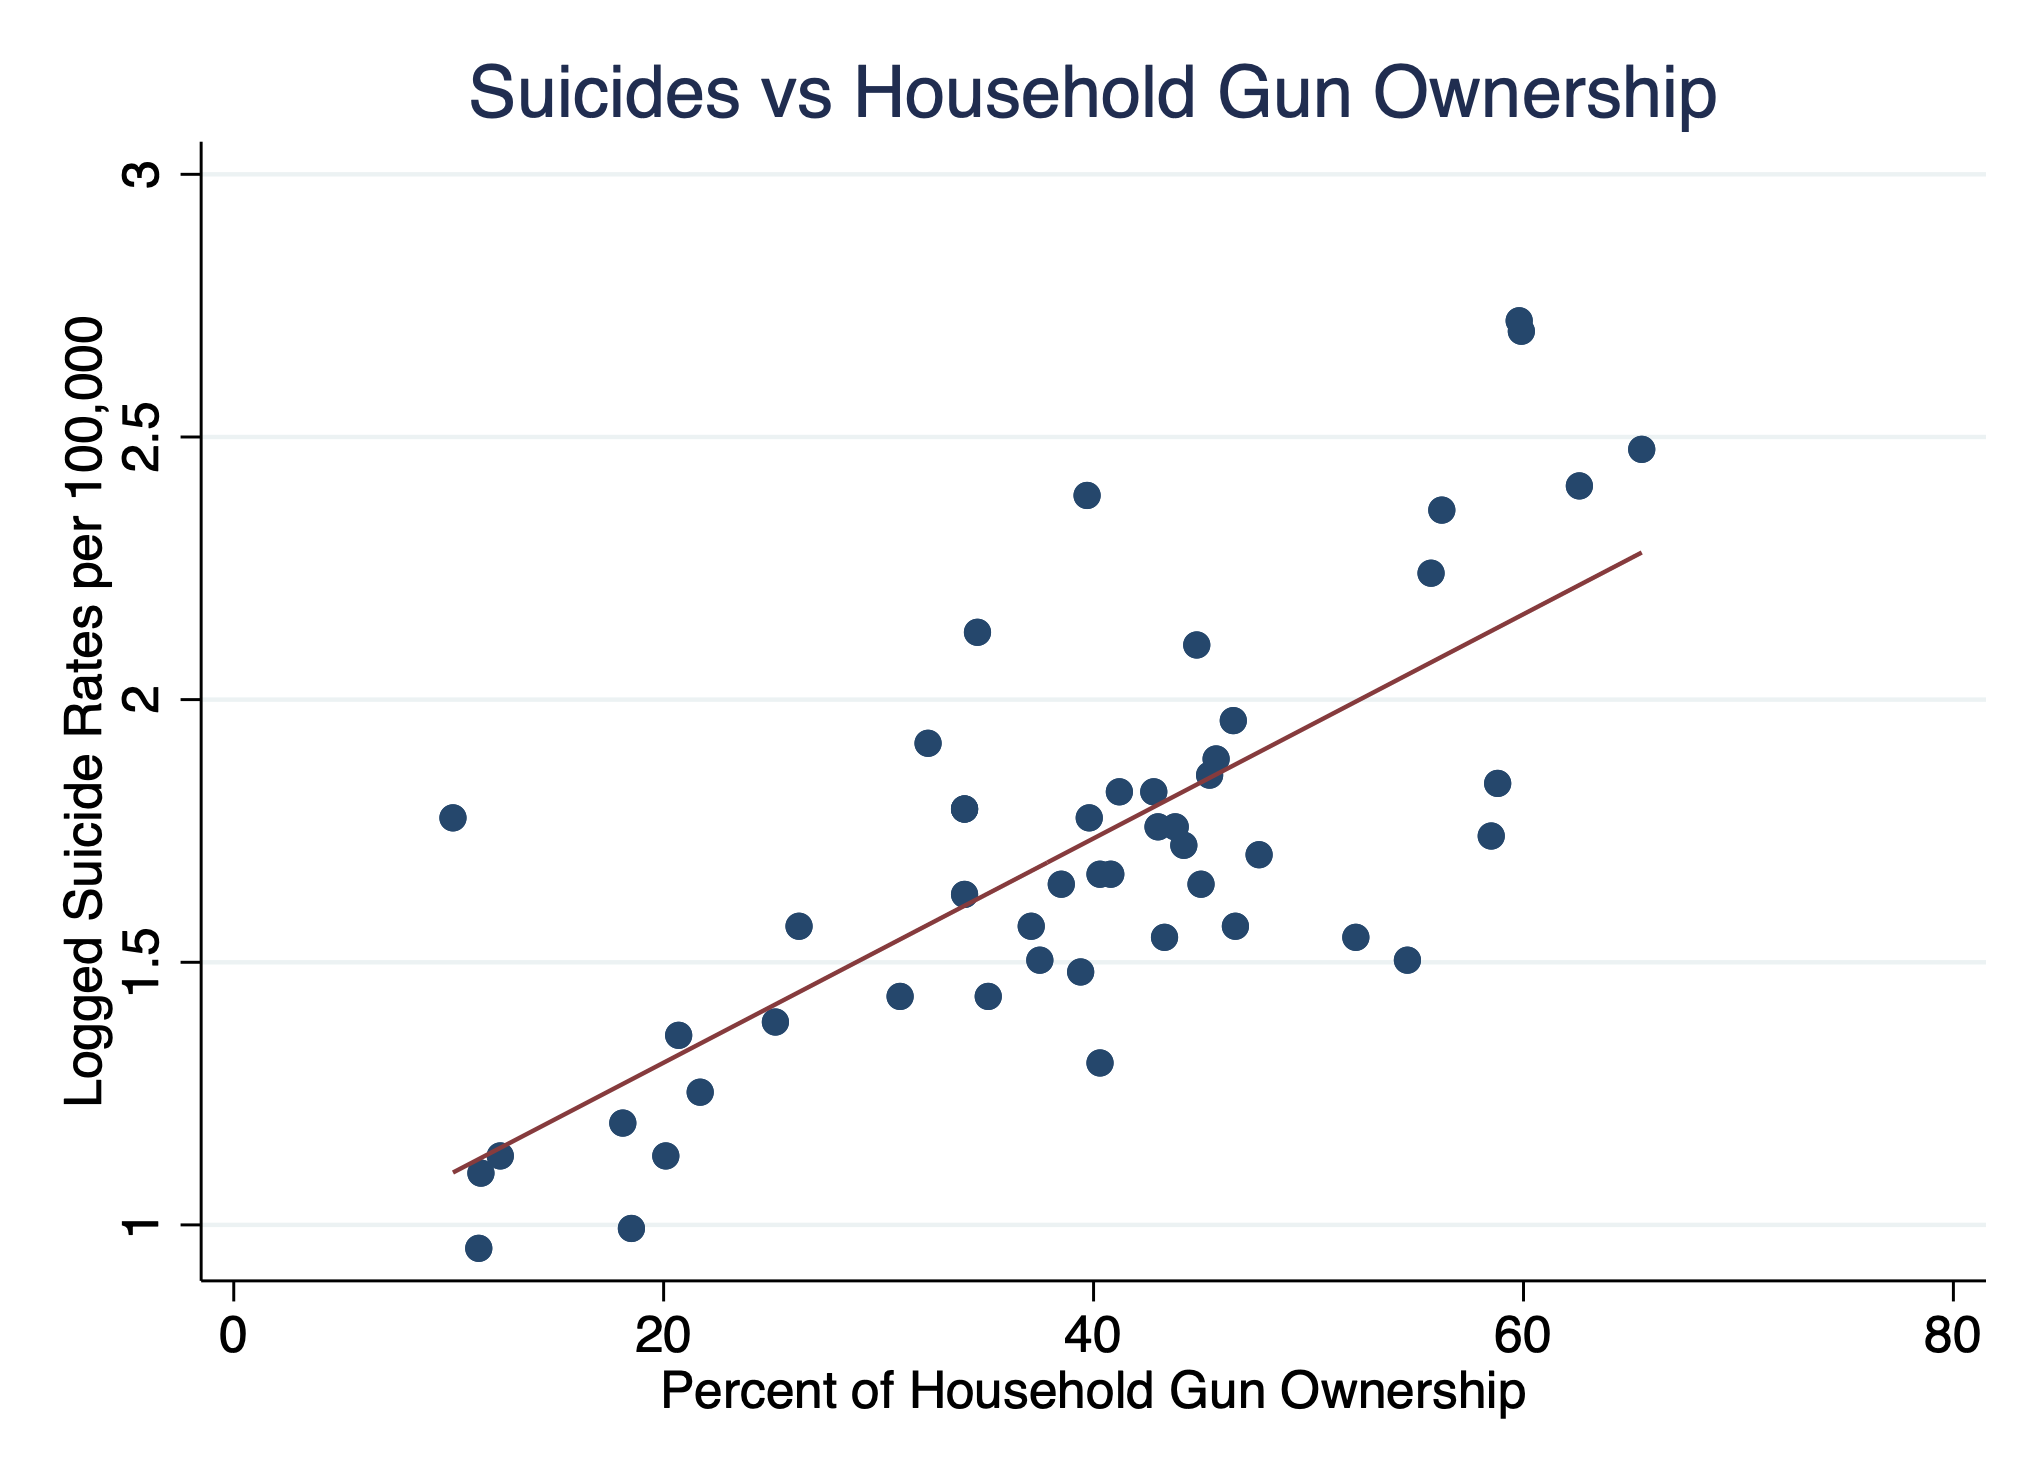
\includegraphics[width=8.5cm]{graph2.png}	
\caption{Correlations between suicide rates and suicide attempts on household gun ownership. On the left, $R^2 = 0.0081$, and on the right, $R^2$}
\end{figure*}



Gun ownership, however, was not a significant predictor $(t = 0.6, p = 0.54)$ of suicide attempts. Therefore while guns are not correlated with overall suicide attempts, they are correlated with successful ones. In Knopov et al (2018), where both gun ownership and suicide attempts was found to be significant in predicting overall suicide, gun ownership was surprisingly the more significant predictor. This is perhaps due to the overwhelming lethality of firearms: as a suicide method, it has 2.6 times the lethality of suffocation,  the second most lethal suicide method. Nevertheless, we could not reproduce the significance of suicide attempts on overall suicides in our data set.\\
\begin{figure*}[h]
\centering	
\begin{verbatim}
	
      Source |       SS           df       MS      Number of obs   =        47
-------------+----------------------------------   F(2, 44)        =     26.98
       Model |  4.51053535         2  2.25526767   Prob > F        =    0.0000
    Residual |  3.67748369        44  .083579175   R-squared       =    0.5509
-------------+----------------------------------   Adj R-squared   =    0.5305
       Total |  8.18801904        46  .178000414   Root MSE        =     .2891

------------------------------------------------------------------------------
  logsuicide |      Coef.   Std. Err.      t    P>|t|     [95% Conf. Interval]
-------------+----------------------------------------------------------------
 logattempts |    .098037   .2445033     0.40   0.690    -.3947271    .5908012
   ownership |   .0213167   .0029323     7.27   0.000     .0154071    .0272263
       _cons |   .6677117   .5259796     1.27   0.211    -.3923306    1.727754
\end{verbatim}
\caption{Logged regression of suicide rates and suicide attempts over gun ownership in 47 states (except Oregon, Minnesota, and Washington).}
\end{figure*}

\subsection*{Discussion}


Higher levels of gun ownership were associated with higher rates of overall youth suicide. This supports the hypothesis that having access to a means of suicide with a high fatality rate increases youth mortality, and that conversely limiting access to firearms, i.e. gun control, is a crucial step in reducing fatalities. The youth in Illinois, for example, attempt suicides (9.1\%) more prevalently than in Iowa (6.6), yet Iowa has a higher suicide rate (6.6 per 100000) than Illinois (3.9\% per 100000), with some of this difference being attributable to there being more household gun prevalence in Iowa (45.7\%) than in Illinois (20.\%).\\

\subsection*{Limitations}

Our study clearly has several limitations. In terms of internal validity, there are problems with the data: the dependent variable, suicide rates, covers youths from the ages 10-19, while in the multiple regression, the independent variable also includes self-reported attempted suicide for youths ages 14-18. However, this should not be a significant problem, as youths aged 10-13 constitute 8\% of the suicides in the dataset. Of the Gauss-Markov assumptions required for estimates from our regression to be BLUE (best linear unbiased estimator), it is almost certain we have violated MR1: proper specification of the function. Omitted variables, which are related to both household gun ownership and youth suicide could bias our coefficient estimates. We attempt to control for this in the  multiple regression of attempted suicides and gun ownership or successful suicides, since the attempted suicides themselves should capture the influences of omitted variables that influence the propensity of a youth to attempt suicide, and we are now approximately estimating the effectiveness of the method itself. Furthermore, as a cross sectional study, causality is not determined; and we cannot say on this study alone, that changes in gun ownership over time within a state will translate into changes in youth suicide rates.\footnote{\#statisticalinference: Explained the importance of proper specification as MR1 of the Gauss-Markov assumptions for the OLS regression being BLUE, including how there was likely omitted variable bias in the simple regression, and how this was addressed in the multiple regression. I also include possible threats to internal validity, such as the mismatch in ages collected for different variables, and why this should not significantly alter our findings. Finally, I establish a significant relationship via a t-test, and contextualize my model.} \\


\subsection*{Conclusion}
Despite the limitations in our study, we find the usefulness of household gun ownership as a predictor of youth suicides at the state level. Specifically, we predict that each 1\% absolute increase in household gun ownership is associated with a 2.15\% relative increase in youth suicides. We hypothesize that the increased prevalence of guns presents a highly lethal option for suicidal teens in order to commit suicide, and thus would suggest public policies to more heavily regulate and reduce access to guns for teens (such as stringent universal background checks, junk-gun bans, permitless carry laws, or even buyback programs) in order to reduce teen mortality.\\

Word Count: 1334, 7 paragraphs, 3 visuals.

\section*{References}

Anestis MD, Selby EA, Butterworth SE. Rising longitudinal trajectories in suicide rates: the role of firearm suicide rates and firearm legislation. Prev Med. 2017;100:159-166. https://doi.org/ 10.1016/j.ypmed.2017.04.032.\\

American Psychology Association (n.d.). Effects of poverty, hunger and homelessness on 
children and youth. Retrieved online from: https://www.apa.org/pi/families/poverty\\

Cash SJ, Bridge JA. Epidemiology of youth suicide and suicidal behavior. Curr Opin Pediatr. 2009;21(5):613-619. https://doi.org/10.1097/ MOP.0b013e32833063e1.\\

Catherine A. Okoro, MS*; David E. Nelson, MD, MPH*; James A. Mercy, PhD; Lina S. 
Balluz, ScD*; Alex E. Crosby, MD, MPH; and Ali H. Mokdad, PhD* (September, 2005). Prevalence of Household Firearms and Firearm-Storage Practices in the 50 States and the District of Columbia: Findings From the Behavioral Risk Factor Surveillance System, 2002. Pediatrics, 116 (3) e370-e376; DOI: https://doi.org/10.1542/peds.2005-0300




\end{document}